
\documentclass[a4paper,10pt]{article}
%\usepackage[left=2cm, right=3cm]{geometry}

\usepackage{fullpage}

\usepackage{tikz}
\usetikzlibrary{shapes, arrows, shadows}

\usepackage{graphicx}

\usepackage{amsmath, amsthm, amssymb,amsfonts}
\usepackage{mathrsfs}
\usepackage{float}
\restylefloat{figure}
\usepackage{pdfpages}

\usepackage{xspace}

\usepackage{color}

\usepackage{xstring}

\usepackage{url}

% some useful math macros (not necessarily needed for this document)
\newcommand{\pd}[2]{\frac{\partial #1}{\partial #2}} % partial derivative
\newcommand{\pdc}[3]{\left(\pd{#1}{#2}\right)_{#3}}  % partial derivative keeping #3 constant
\newcommand{\Dt}{\frac{d}{dt}} % time derivative
\renewcommand{\H}{\mathcal{H}} % Hamiltonian H
\renewcommand{\inf}{\infty}    % infinity
\newcommand{\intinf}{\int_{-\inf}^{\inf}} % integral from -inf  ro inf

% common greek letters
\newcommand{\sig}{\sigma}
\renewcommand{\b}{\beta}
\newcommand{\la}{\lambda}
\newcommand{\si}{\sigma}
\renewcommand{\th}{\theta}
\newcommand{\del}{\delta}
\newcommand{\Del}{\Delta}
\newcommand{\om}{\omega}
\renewcommand{\O}{\Omega}
\newcommand{\ep}{\varepsilon}
\newcommand{\f}{\varphi}
\newcommand{\al}{\alpha}

% useful for equations
\newcommand{\then}{\quad\Rightarrow\quad} % padded double arrow
\newcommand{\with}{\quad\text{with}\quad} 
\newcommand{\an}{\quad \text{and} \quad}  
\newcommand{\comma}{\quad , \quad}

% useful stuff for quantum mechanics
\newcommand{\ket}[1]{|\ #1 \rangle}
\newcommand{\bra}[1]{\langle #1 \ |}
\newcommand{\bracket}[2]{\langle #1 \ | \ #2 \rangle}
\newcommand{\resq}[1]{\tfrac {1} {\sqrt{#1}}}
\renewcommand{\dag}{ ^\dagger}
\newcommand{\levic}[1]{\varepsilon_{#1}}
\newcommand{\comm}[2]{\left[#1\ ,\ #2\right]} % commutator
\newcommand{\mat}[1]{\left(\begin{matrix} #1 \end{matrix}\right)}
\newcommand{\shro}{Shr\"odinger\xspace}

% useful stuff for statistical mechanics 
\newcommand{\ave}[1]{\langle #1 \rangle}
\newcommand{\intdr}{\int d^3 r}
\renewcommand{\deg}{^\circ}


\newcommand{\room}{\vspace{0.3cm}}

\newcommand{\pic}[2][1]{\begin{center}\includegraphics[width=#1\textwidth]{#2} \end{center}}

%%%%%%%%%%%%%%%%%%%%%%%%%%%%%%%%%%%%%%%%%%%%%%%%%%%%%%%%%%%%%%%%%%%%%%%%%%5

% project specific macros:

\newcommand{\arasim}{AraSim\xspace}
%\newcommand{\arasim}{\makebox[.7em]{\raisebox{0.3ex}{A}}\makebox[0.9ex]{\raisebox{-0.2ex}r}\makebox{\raisebox{0.4ex}{a}}\makebox[0.9ex]{\raisebox{0.5ex}{S}}\makebox[0.8ex]{\raisebox{-0.2ex}{i}} \makebox[0.1ex]{\raisebox{0.3ex}{m}}\xspace\xspace\xspace}

% this formats the ARASIM parameters. Don't use '_' it will render them automatically
\newcommand{\p}[1]{\texttt{\StrSubstitute{#1}{ }{\char`_\hspace{0.5pt}}} \xspace} 

% this is used to first define a parameter. same as \p but with reference and spade-suit bullet. Don't use '_' it will render them automatically
\newcommand{\pr}[1]{\vspace{5pt}{\color{blue}$\spadesuit$} \label{#1}\texttt{ \StrSubstitute{#1}{ }{\char`_\hspace{0.5pt}}}} 

%  a reference to a parameter. This is used to print out a short description plus page ref to the guide
\renewcommand{\r}[3][0]{\#\texttt{\StrSubstitute{#2}{ }{\char`_\hspace{0.5pt}}}=#1 // (DEFAULT=#1) #3 \# }

% unused reference to parameters which don't need a reference
\newcommand{\rs}[3][0]{}

% reference section:
\newcommand{\rsection}[1]{\subsection*{\#\#//  #1 (\textbf{user guide}: see section \ref{#1} page \pageref{#1}) //\#}} 

% the emphasis for testbed only! lines
\newcommand{\tb}[1]{{\color{red}\textbf{#1}}} 


% \renewcommand{\labelitemi}{$\clubsuit$}
\renewcommand{\labelitemi}{{\color{black}$\star$}}
\renewcommand{\labelitemii}{{\color{red}$\diamondsuit$}}
\renewcommand{\labelitemiii}{--}

\linespread{1.1}

%%%%%%%%%%%%%%%%%%%%%%%%%%%%%%%%%%%%%%%%%%%%%%%%%%%%%%%%%%%%%%%%%%%%%%%%%%%
%%        *****      BEGIN DOCUMENT       *****                          %%
%%%%%%%%%%%%%%%%%%%%%%%%%%%%%%%%%%%%%%%%%%%%%%%%%%%%%%%%%%%%%%%%%%%%%%%%%%%

\begin{document}
 



\begin{centering}

\title{A Guide to using AraSim}

\noindent\huge \textbf{A guide to using \makebox[.7em]{\raisebox{0.ex}{A}}\makebox[0.6ex]{\raisebox{0.45ex}r}\makebox[0.2em]{\raisebox{-0.3ex}{a}}\makebox[1.0ex]{\raisebox{0.11ex}{S}}\makebox[0.7ex]{\raisebox{-0.3ex}{i}} \makebox[0.0ex]{\raisebox{0.1ex}{m}}}

\normalsize
\room

\author{Guy Nir \\ \small Weizmann Institute, Rehovot}

\Large Guy Nir \\ \small Weizmann Institute, Rehovot

\vspace{0.3cm}

\verb| guy.nir@weizmann.ac.il |

\vspace{1cm}

Based on \arasim software developed at OSU

Special thanks to 

Amy Connolly, Carl Pfendner and Eugene Hong 

for writing this software 

(and the having patience to explain everything to me). 

\room

\today

svn: revision 467

\end{centering}

\vspace{3cm}

\abstract{There are a lot of options to use in AraSim, most of which are not fully documented. I will try to make some short, clear documentation on these functions. I will also try to make clear which options cannot work together and how to get ceratin results by choosing the right parameters.}

Along with this .pdf document is a settings file `setup.txt' which contains the `references' section of this document (section \ref{references} on page \pageref{references}). In it you may find the default values and a quick summary of the different modes for each parameter. 



%\title{\textbf{Title}:\\ some text }

%\author{Guy Nir\\\  \small Weizmann Institute of Science, Rehovot}

%\date{}

%\maketitle 

\room

\newpage

\tikzstyle{decision} = [diamond, draw, fill=blue!50]
\tikzstyle{line} = [draw, -stealth, thick]
\tikzstyle{dline} = [draw, -stealth, thick, double]
\tikzstyle{elli}=[draw, ellipse, fill=red!50,minimum height=8mm, text width=8em, text centered, node distance=7em]

\tikzstyle{desc}=[draw, rectangle, rounded corners, fill=green!60,minimum height=5mm, text width=6em, text centered, node distance=8em]

\tikzstyle{warn}=[draw, rectangle, fill=yellow!90,minimum height=5mm, text width=6em, text centered, node distance=9em]


\tikzstyle{cir}=[draw, circle, fill=red!70, text width=2ex, text centered]


\tikzstyle{block} = [draw, rectangle, fill=blue!50, text width=8em, text centered, minimum height=15mm, node distance=10em]

\tikzstyle{empty}=[node distance=8em]


\section{Compiling Arasim}



\subsection{Prerequisites}

\arasim has a few prerequisists:

\begin{itemize}

 \item sqlite3: useful for reading geometry files. It is important to have this installed and enabled when installing ROOT. 

 \item ROOT: you should already be running root (and, if necessary, have \verb|ROOTSYS| set in your environmental variables). 

 \item Boost: a bunch of libraries for doing things faster in c++: 
 
 \item AraRoot: for the data structures and geometry used in ARA analysis. 
 
 \begin{enumerate} 
  
  \item go to the boost website \verb| www.boost.org | and download the tarball. Untar it to get the source directory. 
  
  \item inside the directory `\verb|boost_x_xx_x/|' do\\ \verb| $ ./bootstrap.sh | and then \verb| $ sudo ./bjam install| 
  
  if you are installing boost on a server/cluster (and can't sudo anything) do
  
  \verb| $ ./bootstrap.sh --prefix=path/to/installation/directory |
  
  \item Add the environmental variables: add to your .bashrc the line:\\ \verb| export BOOST_ROOT=/path/to/boost_x_xx_x/ |
   
 \end{enumerate}

 \vspace{-0.3cm}
 

\end{itemize}

\subsection{Getting the code}

\begin{itemize}

\item To get the latest version of \arasim go to 

\url{http://www.physics.ohio-state.edu/~connolly/AraSim/arainstr.html}

\item or use the svn command\footnote{You may have to do \$ sudo apt-get install subversion} (make sure you `cd' to the place where you want to create the `AraSim/' directory): 

\verb| $ svn --username <yourusername> co https://|

\verb|delos.mps.ohio-state.edu/RadioSim/AraSim/  AraSim | 

(write this in one line). 

\item For more instructions regarding the \arasim svn:

\verb| http://www.physics.ohio-state.edu/~connolly/AraSim/arainstr.html |

\item To get a username and password contact Amy Connolly at: 

\verb| connolly@physics.osu.edu | 

\end{itemize}
 \vspace{-0.3cm}
\subsection{Compiling AraSim from source}

Inside the `\verb|AraSim/|' directory run \verb| $ make | 


Along with \arasim we have two useful programs for looking at the resulting `AraOut.root' file. 

\begin{enumerate} 

 \item readTree.cc: this program makes .pdf files with plots of the waveforms inside the output file. 
 
 do \verb| $ make -f M.readTree | to compile it, then run 
 
 \verb| $ ./readTree | or \verb| $ ./readTree outputs/youroutput.root |
 
 \item readGeom.cc: this program plots the geometry of the detector. 
 
 do \verb| $ make -f M.readGeom | to compile, then run
 
 \verb| $ ./readGeom | or \verb| $ ./readGeom outputs/youroutput.root |
 
\end{enumerate}
 \vspace{-0.3cm}

If any problems arise try the following:

\begin{itemize}

 \item Check the prerequisists and the necessary environmental variables:
 
 \verb| $ echo $ROOTSYS| should give the directory of ROOT (this may not work in fixed location installation method of ROOT). 
 
 \verb| $ echo $BOOST_ROOT| should point to the boost directory. Make sure the distribution number is right (latest is `\verb|boost_1_54_0|' as of this article). 
 
%  \item Check that the makefile has:
%  
%  \begin{itemize}
%  
%  \item in the \verb| SYSLIBS| line make sure \verb| -L/usr/local/lib | appears after \verb| -L/usr/lib| 
%  
%  \item in the \verb| LDFLAGS| line make sure \verb| -lAraGeom | appears after \verb| -lAraSimEvent|
%  
%  \item in the \verb| $(DL) $(LDFLAGS) | line make sure \verb| -lAraGeom | and \verb| -lsqlite3 | appears after \verb| -lAraSimEvent |. 
%  
%  \end{itemize}
 
 \item If all else fails: contact Eugene Hong (\verb| ripple90@gmail.com |), Carl Pfendner\\ (\verb| pfendner.1@physics.osu.edu |) or Amy Connolly. 
 
\end{itemize}

\pagebreak


\tikzstyle{quest} = [draw, rectangle, fill=blue!20, text width=8em, text centered, minimum height=15mm, node distance=10em]

\begin{figure}[H]
 
 \room
 
 \begin{centering}
  
  \begin{tikzpicture}[scale=0.5]
   
   
   
   \node[block] (problem) {I have a problem};
   
   \node[quest, below of=problem, yshift=4em] (read?) {Is it in the manual?};
   
   \path[line] (problem) -- (read?);
   
   \node[quest, left of=read?, xshift=-8em] (not in manual?) {Is it something that \emph{should} be in the manual?};
   
   \path[line] (read?) --node[cir, text width=2em]{no} (not in manual?);
   
   \node[quest, below of=read?] (understand?) {Did you understand what was written?};
   
   \path[line] (read?) --node[cir, text width=2em]{yes} (understand?);
   
   \node[desc, below of=not in manual?, text width=12em, yshift=-2em] (call guy) {Send an email to \texttt{guy.nir@weizmann.ac.il}};
   
   \path[line] (understand?) --node[cir, text width=2em] {no} (call guy);
   
   \path[line] (not in manual?) --node[cir, text width=2em]{yes} (call guy);
   
   \node[empty, left of=not in manual?] (around) {};
   
   \node[block, below of=understand?, text width=20em] (clear) {Everything is perfectly clear in the manual, but I still have a problem with...};
   
   \path[line] (understand?) --node[cir, text width=2em] {yes} (clear);
   
   \path[line] (not in manual?) --node[cir, text width=2em, xshift=-2em] {no} (around) |- (clear);
   
  
   \node[quest, fill=red!70,below of=clear, xshift=2em, yshift=-2em] (run it) {I can't get it to run at all...};

   
  \node[quest, fill=red!70,right of=run it] (physics) {The physics used is not clear to me...};

  \node[quest, fill=red!70,left of=run it] (new func) {I need new functionality that doesn't exist in the current \arasim};

  \node[quest, fill=red!70,left of=new func] (flowcharts) {I don't know how to read flowcharts...};
 
  \path[line] (clear) -- (flowcharts);
  
  \path[line] (clear) -- (new func);
  
  \path[line] (clear) -- (run it);
  
  \path[line] (clear) -- (physics);
 
  \path[line] (flowcharts) -- (call guy);
  
  \node[desc, below of=run it, text width=12em, yshift=-2em] (eugene) {Send an email to Eugene Hong: \texttt{ripple90@gmail.com}};
 
 \path[line] (new func) -- (eugene);
 \path[line] (run it) -- (eugene);
 \path[line] (physics) -- (eugene);
 
     
   
  \end{tikzpicture}

  
  
 \end{centering}


 
 \caption{What to do in case you have any trouble with \arasim}
 
  \label{problems flowchart}
 
 \room
 
\end{figure}









\newpage

\section{Using Arasim}\label{running arasim}

\subsection{Basic implementation}\label{basic implementation}

Once \arasim is compiled we can run it by doing \verb| $ ./AraSim| which runs the simulation using the default setup file `setup.txt'. If this file has not been changed \arasim should run 100 neutrino events (not a very long simulation). 

The primary output of \arasim is through an output file found in `outputs/AraOut.root'. This contains three trees: 

\begin{itemize}

 \item AraTree: contains the global parameters of the run, such as the detector setup, the neutrino energy spectrum and the earth and ice models used in the simulation. 
 
 \item AraTree2: contains detailed information for each seperate event, such as the position of the interaction vertex, the energy of each simulated neutrino, and lots of other information on the specfic event. 
 
 \item eventTree: This tree contains the data that would be available in real analysis. It simulates the data structures we would get from a real detector. It should have the waveforms as they are picked up by the antennas, and some other information measureable by the detector. 
 
 
\end{itemize}

Depending on the data saving mode, these trees may contain more or less data. By default the `AraTree2' should contain all events generated while `eventTree' should have data only for globally triggered events. 

\room

\subsection{Advanced users}\label{advanced users}

After making sure \arasim works well, we should customize the simulation to our own needs. The simplest way to do this is to change parameters inside `setup.txt'. Once changes are made to this file a new simulation can be run, with the output file being overwritten by the new `AraOut.root' file. For more explanations on what parameters we can change in a setup file, see section \ref{setup file}.

For serious use of \arasim, we strongly recommend to generate renamed copies of `setup.txt', for example `setup.example.txt'. Running \verb| $ ./AraSim setup.example.txt | will use the settings inside this new file. 

As a practical example, we may have `setup.TB.txt' and `setup.ARA37.txt' which we run one after another, the first with testbed parameters, and the second with a large detector. This lets us keep several sets of our favourite parameters without needing to constantly comment out and rewrite values. 

\room

If we don't want our output files to overwrite each time we run \arasim, we should specify as inputs for \arasim not just the setup file, but also a run number. For example:

\verb| $ ./AraSim setup.TB.txt 3 | 

will run \arasim using the testbed parameters inside `setup.TB.txt' and save the output to `outputs/AraOut.setup.TB.txt.run3.root'. 

We may use this functionality for running \arasim as a real detector, which generates several runs (it will also allow us to start analysis on the first files before all the simulations are done). Instead of running one simulation with $10^6$ neutrinos we may run ten simulations of $10^5$ neutrinos each, and get ten output files:

\verb| $ for i in `seq 1 10` ; do ./AraSim setup.txt $i ; done |

should generate ten files `outputs/AraOut.setup.txt.\#.root', that can be loaded into a chain just like real detector data. 

\room

Another useful possiblity is to run simulation on several setup files, saving the output to different output files without necessarily changing the run number:

\verb| $ ./AraSim setup.TB.txt 0|
\verb| $ ./AraSim setup.ARA37.txt 0|

will give us two different outputs, one for each detector setup, both at run number 0. 

For setup files that are inside subfolders or on a completely different path, AraSim will truncate the path to the setup file when writing the output files, e.g.:

\verb| $ ./AraSim SETUP/parameter/setup.par.txt 0 | will create output file: 

\verb| AraOut.setup.par.txt.run0.root | and not the entire path. 

\room

If you wish to specify the output directory for \arasim, simply add the path after the run number:

\verb| ./AraSim setup.txt 0 /some/other/path/to/store/outputs/ |

This is especially useful when running large data sets that do not fit in a user's home directory. 

\subsection{Super users}\label{super users}

For running massive simulations we recommend setting up \arasim on a cluster, where we can send multiple jobs to run. This allows us to run multiple simulations at once, freeing our computer and our time to write user guides for simulation programs. 

Depending on the super computer / cluster used we recommend using some queue submission e.g.

\verb| for i in `seq 0 99`; do qsub -v var=$i ./run_sim.sh | 

(Additional options may include \verb| -N job_name |, \verb| -k oe | (error and output redirection), and \verb| -q which_queue |  depending on the system). 

\room

The script \verb|run_sim.sh| can do something like:

\verb| #!/bin/bash  //  ./AraSim setupfile $var | 

along with additional scripts to redirect outputs to logfiles, move the output files etc. 


Make sure you ask your local cluster admin for instructions on how to submit multiple jops to the grid. 

\room

In any case, the outputs of running \arasim on several machines will all funnel back into the \verb|outputs/| directory, unless you specified a different output (i.e.~some hard drive that can store large data sets instead of the home directory). If you do multiple runs with a distinct setup file and run number you can gather them all up at the end (or even after a few finished runs) and start analysis. 


\room

\subsection{Data Analysis}

Analizing the data from \arasim output files divides into two categories. There is the `behind the scenes' information such as the position of the interaction vertex and the energy of the incoming neutrino, and there is the `real data' which mimicks the output of a real detector (waveforms primarily). 

\room

As explained in section \ref{basic implementation} there are two trees for `behind the scenes' information. Most the information in `AraTree' is stored in the Detector and Settings classes. The specific events (kept in `AraTree2') are accessible via the Event and Report classes. 

\room

The detector style information is saved in `eventTree', using classes from AraRoot (version 3.13), i.e.~`UsefulIcrrStationEvent'. 

% Make sure you load the right headers and libraries from the \arasim directory, not from AraRoot. It may be necessary to compile a dynamic library containing the \arsim and AraRoot3.2 classes. 

% This should include \verb| Detector.o  EarthModel.o  Ray.o | etc.~as well as the AraRoot formats for geometry: inside \verb| AraRoot/ | we have \verb| AraGeomTool.o  AraStationInfo.o | etc.~and for event class inside \verb| AraRootFormat/ | we need \verb| UsefulIcrrStationEvent.o |. \

% You may have these libraries loaded in your makefile. For use with \verb|g++| directly, make a new library name \verb|libSim.so| using:

% \verb< gcc -shared -Wl,--no-as-needed  $(ls | grep '^[^A]*\.o' | tr '\n' ' ')< //

% \verb< $(ls AraRoot | grep '\.o$' | awk '{print "AraRoot/" $1}'| tr '\n' ' ') < //

% \verb<$(ls AraRootFormat | grep '\.o$' | awk '{print "AraRootFormat/" $1}'| tr '\n' ' ')<//

% \verb< -o libSim.so<  

If you have analysis code that depends on the AraSim library, you may wish to generate a dynamically loaded library that knows all the classes used by \arasim. Use \verb| ./library.sh | to create \verb| libSim.so |. You can now compile any code with the AraSim headers, and link to this library. Make sure it is in your \verb| LD_LIBRARY_PATH |

example:

% when inside the \arasim directory. This \verb|.so| file should contain all the relvant classes to run scripts for data analysis. Example:

\verb| g++ example_loop.cxx -I$SIM -I$SIM/AraRoot -I$SIM/AraRootFormat| //

\verb| -L$SIM -lSim `root-config --cflags --libs` -o program.exe |

Where \verb| $SIM| is the directory of AraSim. This program can have access to the trees inside the \arasim output files, reading geometry, event physics and the actual waveforms similarly to the way we access L0 files in AraRoot (with Iccr rather than the newer Atri board). Make sure you actually write the waveforms to file (see section \ref{writing events}).

% Make sure \verb|libSim| is in your \verb|LD_LIBRARY_PATH| when running any such code. 

\newpage


\expandarg %for the xstring package and expanding the underscores

\section{Simulation Modes and Parameters} \label{setup file}

Each simulation is made using the parameters found in `setup.txt'\footnote{As explained in section 
\ref{super users} it is advisable to make differently named copies of `setup.txt' and run `\$ ./AraSim yoursetup.txt' }  . Although some explanations are found in comments within the file itself, and some are self-explanatory, a more detailed explanation for each parameter is given below. 

\room

These parameters are read into the \verb|Settings| class. If any field is commented out or removed from the setup file, default values are used (as defined in `Settings.cc'). 

\room 

You may comment out any part of the `setup.txt' file using `\verb|//|'. 

Adding lines like this: `\p{PARAMETER}= N' will set the appropriate parameter to N. The order of input lines is irrelevant, but if two or more lines set the same parameter, the last one will be used. 

\subsection{Neutrino energies}\label{neutrino energies}

\setlength{\parindent}{0pt}

\pr{EXPONENT}=19. This determines the energy spectrum of the incoming neutrinos. 

For selecting a single energy choose values \p{EXPONENT}= $N$. When $10<N<20$, \arasim will generate neutrinos with energies $E=10^N$eV. Taking values too low or too high may lead to strange results in the simulation (The ARA detector should work well for neutrinos at energies of $E\sim 10^{15} - 10^{20}$eV only). 

In order to simulate real spectra of neutrinos, so each neutrino energy is randomly chosen from a distribution of energies, use \p{EXPONENT}= $N$ with values $1<N<4$, or $N\geq30$. 

For $1<N<4$ the distribution is just $E^{-N}$. 

% Choosing $N\geq20$ gives energies based on different models (see list\footnote{Work in progress. Use `README\textunderscore~EXPONENT.pdf' for more details}).

If you wish to give a more specific energy value to all neutrinos, use $510\leq$ \p{EXPONENT}$\leq 650$, AraSim will give an energy of $10^x$~eV to all neutrinos, where $x=(\p{EXPONENT}-400)/10$. For example, to get $E=10^{18.3}$~eV neutrinos, use \p{EXPONENT}= 583.


\room

To generate neutrinos at random energies from specific distributions (flux models) use \linebreak $30\leq \p{EXPONENT}\leq 500$. The specific choice of flux model can be examined in `Spectra.cc', with some of the flux model files stored in \verb| fluxes/ |.






\newpage

\subsection{The number of neutrinos simulated}\label{number of neutrinos}


\pr{ONLY PASSED EVENTS}=0. Choosing the number of neutrinos generated in the simulation can be made in two ways. If we choose \p{ONLY PASSED EVENTS}= 0 then we can specify how many $\nu$'s to generate in the simulation. Thus the total time of simulation is known \emph{a-priory} but the number of $\nu$'s globally triggered can vary (can even be zero). 

\pr{NNU}=100. In this case (\p{ONLY PASSED EVENTS}= 0) the number of neutrinos generated should be specified in \p{NNU}= \emph{(\# of neutrinos)}.

\room 

The second option is \p{ONLY PASSED EVENTS}= 1, where we specify how many $\nu$'s pass the trigger. \arasim will generate as many $\nu$'s as necessary until the requested number is reached. In this mode the size of the sample that will trigger is known in advance but the run time may vary. If reasonable parameters are not chosen, the run time may be very long. 

\pr{NNU PASSED}=0. When using this mode (\p{ONLY PASSED EVENTS}=1), \arasim will ignore the \p{NNU} field and look instead at \p{NNU PASSED}. This field determines how many neutrinos will globally trigger. 

\pr{OUTPUT TDR GRAPH}=0. Saves this number of tunnel diode response (TDR) waveforms for debugging. 

\begin{figure}[H]

\room

\begin{centering}

\begin{tikzpicture}
 
 \node[block] (only passed){\p{ONLY PASSED EVENTS}};
 
 \node[below of=only passed, yshift=-5em] (middle){};
 
 \node[block, left of=middle] (nnu) {\p{NNU=100}};
 
 \node[block, right of=middle] (passed) {\p{NNU PASSED=10}};
 
 \node[desc, below of=nnu] (nnu desc) {\arasim will generate exactly this many $\nu$'s};
 
  \node[desc, below of=passed] (passed desc) {\arasim will generate $\nu$'s until this many have triggered};
 
 %arrows
 
 \path[dline] (only passed) --node[cir]{0} (nnu);
 
 \path[line] (only passed) --node[cir]{1} (passed);
 
 \path[dline] (nnu) -- (nnu desc);
 
 \path[line] (passed) -- (passed desc);
 
 \node[warn, left of=only passed, xshift=-5em, yshift=-1em, minimum height=8em, text width=12em] (rectangle) {};
 
 \node[left of=only passed, xshift=-10em, yshift=2em, minimum height=3cm, text width=12em] (legend) {\textbf{legend:}};
 
 \node[empty, left of=legend, yshift=-2em, xshift=4em] (left1) {}; 
 
 \node[empty, left of=legend, yshift=-6em, xshift=4em] (left2) {}; 
 
 \node[empty, right of=legend, yshift=-2em, xshift=-4em] (right1) {}; 
 
 \node[empty, right of=legend, yshift=-6em, xshift=-4em] (right2) {}; 
 
 \path[dline] (left1) --node[yshift=1em]{default} (right1);
 
 \path[line] (left2) --node[yshift=1em]{alternative} (right2);

\end{tikzpicture}

\room

\end{centering}


\caption{Decision on number of neutrinos to generate}

\label{nnu flowchart}



\end{figure}

\newpage


\subsection{Generating noise}\label{generating noise}

\pr{NOISE EVENTS}=16. The number of noise waveforms to be generated as background for the signal. 

\pr{NOISE WAVEFORM GENERATE MODE}=0. In the old versions of \arasim, noise waveforms were generated before the simulation. Now we have as default \p{NOISE WAVEFORM GENERATE MODE}= 0, which generates new noise waveforms for each event. In this mode we need to specify the number of noise waveforms used for each event, so that \p{NOISE EVENTS} should be set to the number of channels used in each station. More noise events are not used. If less \p{NOISE EVENTS} are generated then they are recycled within an event (not good for us).

If you really want to work in the old methods choose \p{NOISE WAVEFORM GENERATE MODE}= 1 and choose \p{NOISE EVENTS} to be a large number, enough to provide \arasim with enough noise events to use when generating all events. 


\pr{NOISE}=0 (default) generates waveforms from a flat thermal distribution. mode 1 uses calibrated Rayleigh distribution noise from testbed data (only used for lower 8 channels - see triggering~\ref{triggering}). 

\pr{NOISE TEMP MODE}=0 (default) generate the same noise waveforms for all channels. When using \p{NOISE}= 1 (Rayleigh distribution), we can choose several modes: mode 1 generate different noise temperatures for each channel; mode 2 generates different noise for the first 8 channels (borehole antennas) and the rest are all the same.  

\pr{NOISE TEMP}=325. If the noise is generated from a thermal distribution (\p{NOISE}= 0), then the temperature of the noise is determined by \p{NOISE TEMP} (default is 325) given in Kelvins. This value is composed of the ice temperature ($T_{ice}=230$K) added to the receiver noise ($T_{rec}=95$K).  

\pr{DATA BIN SIZE}=16384. This must be a power of 2. This field is the length of the noise waveforms that are generated before simulation starts. It is used for the old method where all noise waveforms are pregenerated (in \p{NOISE WAVEFORM GENERATE MODE}= 1). \emph{Also} we use this size in the new mode only to set the \emph{noise floor} by generating a number of noise waveforms of this length and calculating their RMS. 


\begin{figure}[H]

\room

\begin{centering}
 
 \begin{tikzpicture}
  
  \node[block] (noise) {\p{NOISE}};
  
  \node[below of=noise,yshift=-4em](middle) {};
  
  \node[block, left of=middle ] (noise temp) {\p{NOISE TEMP}= 325};
  
  \node[block, right of=middle] (noise temp mode) {\p{NOISE TEMP MODE}};
  
  \node[desc, below of=noise temp] (noise temp desc) {flat thermal noise in the given temperature};
  
  \node[desc, below of=noise temp mode](mode 1){different settings for each channel};
  
  \node[desc, left of=mode 1](mode 0){same noise for all channels};
  
  \node[desc, right of=mode 1](mode 2){different noise for first 8 channels (BH antennas)};
  
  \node[warn, right of=noise,xshift=1em,yshift=0em] (tb only) {\tb{Testbed only!}};
  
  \node[below of=mode 2, yshift=-1.5em, xshift=4em] (below) {};
  
  \node[below of=tb only, yshift=-0.4em] (under) {};
  
%   \draw[style=dashed] (-1,-1) rectangle (8,-6.5);

  \draw[style=dashed] (-1,-1) rectangle (below);
  
  
  
  \draw[style=dashed] (tb only) -- (under);
  
   %arrows
 
%  \path[line, dashed] (tb only) -| (mode 0);
 
 \path[dline] (noise) --node[cir]{0} (noise temp);
 
 \path[line] (noise) --node[cir]{1} (noise temp mode);
 
 \path[dline] (noise temp) -- (noise temp desc);
 
 \path[line] (noise temp mode) --node[cir]{1} (mode 1);
 
 \path[dline] (noise temp mode) --node[cir]{0} (mode 0);
 
 \path[line] (noise temp mode) --node[cir]{2} (mode 2);
 
 \end{tikzpicture}


 
 \caption{Decision on what noise to generate}
 
  \label{noise flowchart}
 
\end{centering}


\end{figure}


% flowchart of NOISE NOISE_TEMP_MODE and NOISE_TEMP

\newpage

\subsection{Position of simulated neutrino}\label{neutrino position}

\pr{INTERACTION MODE}=1. \arasim generates a random position for the interaction of the neutrino based on the choice made for \p{INTERACTION MODE}:

\begin{itemize}

%  \item \textbf{Pick unbiased} (mode 0): chooses a random location in the antarctic ice sheet. May lead to many neutrinos being outside the range of the detector. 
 
 \item \textbf{Aeff mode (spherical volume)} (mode 0): choose neutrino location in sphere around detector, but only inside ice. Makes an unbiased sample of events so we can get the effective area directly. This automatically chooses the new \p{GET CHORD} mode. Make sure you set \p{POSNU RADIUS} to 5km (or more) for this mode. 
 
 This mode has the advantage that it already takes into account the survival probability of neutrinos passing through the earth. 
 
  
 \pr{POSNU RADIUS}=3000, in meters. Determines the radius around the detector in which the neutrinos are generated.
 
   Make sure you choose a reasonable radius for the position of the neutrino interaction. If you choose a large detector, for example ARA37, make sure you increase the size of \p{POSNU RADIUS} to include the detector and the area around it (for ARA37 consider using $\sim$13000)

 \room
 
 \item \textbf{Veff mode (cylindrical volume)} (mode 1, default): Chooses $\nu$ interaction position close by to the detector, within a cylinder of radius R. In this mode we get the effective volume. This uses the old \p{GET CHORD} function. 

 
 \pr{PICK POSNU DEPTH}=0 (default) takes all the ice down to the bedrock (according to the earth model used). mode 1 allows the user to choose a maximum depth for the position of the neutrinos. 
 
 \pr{MAX POSNU DEPTH}=200 in meters depth. When the above is set to mode 1, use this to determine the maximum depth of the position of the generated neutrino. 
 
\room
 

 \item \textbf{Pick exact} (mode 2): this chooses the position of all $\nu$'s to be at the same location. The position of interaction is built into \arasim at this time (look inside `Primaries.cc' for \p{INTERACTION MODE}==2). 
 
 The position given by default is at $R=1000$m, $\th=-\pi/4 $ and $\phi=-\pi/6 $, which translates into 
  \begin{equation*}  
  x=353.55 \text{m} \quad y=612.37\text{m} \quad z=707.1\text{m}
   \end{equation*}
  

   relative to the station center. This mode is useful for testing reconstruction at a specific location, or for making sure all events have a ray trace solution (see subsection \ref{ray solving}).
   
%    \item \textbf{Pick near-unbiased} (mode 3): choose position of $\nu$'s in a sphere around center of ARA stations. 
   
%    \underline{in pick near-unbiased mode only}:
   
%    \pr{PICKNEARUNBIASED R}=5000 the radius around detector when using above mode 3. This is far enough to contain all relevant events when using single station. Like \p{POSNU RADIUS}, make sure you choose a larger size when using multiple stations. 



\end{itemize}



The direction of the incoming neutrino can be predetermined using

\pr{NNU THIS THETA}=0 (default) chooses randomly any angle within the range $\th\in [0,\pi]$. mode 1 lets you choose a specific value for $\th$ and some range around that angle. 

\pr{NNU THETA}=0.785 in radians (=45$^\circ$) the angle chosen when using \p{NNU THIS THETA}= 1. 

\pr{NNU D THETA}=0.0873 in radians (=5$^\circ$): the variability above and below the chosen $\th$, when using \p{NNU THIS THETA}= 1.

\room

\pr{SECONDARIES}=1. mode 0: does not allow any more interactions after the first. mode 1 (default): allow secondary interactions.

\pr{TAUDECAY}=1. mode 0: do not allow secondary $\tau$ particle decays. mode 1 (default): let $\tau$ particles that are generated from $\nu_\tau$ to also have a secondary decay in the ice. Only works when \p{SECONDARIES} is set to 1. 



\newpage

\subsection{Ray Solving}\label{ray solving}

\pr{RAYSOL RANGE}=5000 in meters. Each neutrino event is generated at a certain distance from the detector (see subsection \ref{neutrino position}). Before the event is tested for triggering it is tested for plausible ray trace solution. This is simply done by comparing the distance of the position of the neutrino \p{(POSNU)} from the station center to a radius given by \p{RAYSOL RANGE}. If the neutrino is generated outside of \p{RAYSOL RANGE} then \arasim will not test the trigger and just assume there is no ray solution. 

For a single station, make sure this is larger than \p{POSNU RADIUS} in `pick near', and larger than the default 1000m radius for `pick exact'. 

For multiple stations this test is done for each station seperately, before each station tests for trigger. 

\subsection{Simulation mode}

\pr{SIMULATION MODE}=0 (default) uses frequency domain simulations (AVZ parametrized mode in frequency domain). mode 1 uses the new time domain simulation. The new simulation mode is more realistic and takes between 1.5 to 2 times longer. Also, expect less triggers (as the signal gets more dispersed and has a lower chance of triggering enough channels). 

for time domain (\p{SIMULATION MODE}=1) only:

\pr{SHOWER MODE}=2. Decides on hadronic / EM showers. 0: EM shower only, 1: hadronic shower only. 2 (default): use either EM or HAD shower, depending on signal strength. 

\pr{SHOWER STEP}=0.001 This decides the physical step size (in meters) for the simulation. Default 1mm is small enough for most applications. 

\pr{SHOWER PARAM MODEL}=0 Shower parameters, choose between 0: Jaime's fit, 1: Carl's fit. 

\pr{OFFCONE LIMIT}=10 (degrees). This limits calculations of radiation more than 10 degrees (default) away from the Cherenkov angle, in order to save calculation time where the emitted radiation is already very weak. 


%FLOWCHART of ray solving and triggering and saving

\tikzstyle{action}=[draw, rectangle, rounded corners, fill=red!40,minimum height=5mm, text width=15em, text centered, node distance=6em]

\begin{figure}
 
 \room
 
 \begin{centering}
  
  \begin{tikzpicture}
   
   \node[action] (generate noise) {Generate noise waveforms and get diode RMS response}; 
   
   \node[action, below of=generate noise, yshift=2em] (start) {Generate a neutrino interaction};
   
   \node[block, below of=start, yshift=6em] (interaction) {\p{INTERACTION MODE}};
   
   \path[line] (generate noise) -- (start) ;
   
   \path[line] (start) -- (interaction);
   
   \node[empty, right of=start, xshift=7em] (mid2) {};
   
   \path[line] (mid2) --node[yshift=1.1em]{neutrino event loop} (start);
   
   \node[desc, left of= interaction, xshift=-4em, text width=10em] (desc interaction) {This mode decides the location of the generated interaction};
   
   \path[line] (interaction) -- (desc interaction);
   
   \node[action, below of=interaction] (raysolve) {Check to see if there is a ray trace solution};
   
   \path[line] (interaction) -- (raysolve);
   
   \node[block, below of=raysolve, yshift=5em] (raysol radius) {\p{RAYSOL RADIUS}};
   
   \path[line] (raysolve) -- (raysol radius);
   
   \node[desc, left of=raysol radius, xshift=-4em, text width=12em] (desc raysol radius) {Any neutrinos generated outside this radius are automatically rejected};
   
   \path[line] (raysol radius) -- (desc raysol radius);
   
   \node[action, below of=raysol radius, yshift=1em] (do raytrace) {Check \p{RAYSOL RADIUS} then use ray tracing algorithm. Are there any solutions?};
   
   \path[line] (raysol radius) -- (do raytrace);
   
   \node[action, below of=do raytrace, yshift=-2em, text width=20em] (apply detector) {Apply detector components onto spectrum to get signal waveforms};
   
   \path[line] (do raytrace) --node[cir, text width=2em]{yes} (apply detector);
   
   \node[empty, right of=do raytrace, xshift=7em] (mid3) {};
   
   \path[line] (do raytrace) --node[cir]{no} (mid3);
   
   \path[line] (mid3) -- (mid2);
   
   \node[block, below of=apply detector, yshift=5em] (trigger mode) {\p{TRIG ANALYSIS MODE}};
   
   \path[line] (apply detector) -- (trigger mode);
   
   \node[empty, below of=trigger mode, yshift=4em] (mid4) {};
   
   \node[action, right of=mid4, xshift=3em, yshift=-6em, text width=8em] (just signal) {Add signal to zero waveforms};
   
   \path[line] (trigger mode) -|node[cir]{1} (just signal);
   
   \node[action, left of=mid4, xshift=-2em, yshift=-1em, text width=6em] (make noise) {Generate enough long noise waveforms};
   
   \node[desc, left of=trigger mode, xshift=-10em, text width=10em] (desc trigger) {mode 0 (default): noise+signal \\ mode 1: noise only \\ mode 2: signal only};
   
   \path[line] (trigger mode) -- (desc trigger);
   
   \path[line] (trigger mode) -|node[cir, text width=2em]{0,2} (make noise);
   
   \node[empty, below of=make noise] (mid5) {};
   
   \node[empty, below of= trigger mode, yshift=-4em] (last mid) {};
   
   \node[action, left of= mid5, yshift=3em, text width=9em] (add signal) {Add signal on top of noise waveforms};
   
   \path[line] (make noise) -|node[cir]{0} (add signal);
   
   \path[line] (add signal) |- (last mid);
   
   \node[action, below of=last mid, yshift=1em, text width=20em] (check) {Check if waveforms passed trigger};
   
   \path[line] (make noise) -|node[cir]{2} (check);
   
   \path[line] (just signal) |- (last mid);
   
   \node[empty, right of= check, xshift=7em] (mid1) {};
   
   \path[line] (check) --node[yshift=-2em, text width=6em, text centered]{didn't pass global trigger} (mid1);
   
   \path[line] (mid1) -- (mid3);
   
   \node[action, below of=check] (write) {Write event to file (see section \ref{writing events})}; 
   
   \path[line] (check) --node[xshift=0em, text centered]{passed trigger} (write);
   
  \end{tikzpicture}


  
  \caption{\arasim basic flowchart}
  
    \label{basic flowchart}
  
  \room
  
 \end{centering}

 
 
\end{figure}

\newpage

\subsection{Triggering}\label{triggering}


\pr{USE INSTALLED TRIGGER SETTINGS}=0 (default) this tells \arasim to use the ideal detector setup for triggering. mode 1 future release. %uses the triggering as it is implemented in the actual stations. 

\pr{TRIG ANALYSIS MODE}=0. There are three options to choose:

\begin{itemize}

  \item Signal+Noise (mode 0, default): \arasim will look at noise and signal when deciding if an event triggers or not (this is the realistic mode).
  
  \item Signal only (mode 1): In this mode the noise is not added to the event waveform. This allows us to see exactly where the peak of the signal is, without any distracting noise. Note: the waveform saved will not have any noise in it (clean signal). 
  
  \item Noise only (mode 2): Here we do not add the signal to the waveforms and check to see if the alone noise passes the trigger. This is useful for simulating min-bias (forced) trigger. Note: the waveforms saved will conatin just noise. 
  
  To use this mode make sure you choose the position of the interaction (see \p{INTERACTION MODE} in subsection \ref{neutrino position}) to be close to the station (or use \p{CALPULSER ON} $> 0$ for testbed) so that all events have a ray tracing solution. This ensures every event manages to reach the trigger check (since there is no signal in this mode the distance to the detector is relevant \emph{only} for the ray tracing solution check).
 
  \end{itemize}

\pr{POWERTHRESHOLD}=-6.15. To determine if an event has passed the trigger, \arasim looks at several parameters. The first is \p{POWERTHRESHOLD}. This number determines how strong an event is compared to the noise RMS. A value of \p{POWERTHRESHOLD}= -5 means that a signal needs to be five $\sigma$ stronger than the noise (five times stronger than the noise RMS). This is always given in negative numbers. The closer you are to zero the weaker the trigger threshold. 

Default is \p{POWERTHRESHOLD}= -6.15 similar to the 100 Hz trigger rate of the actual stations. 

\pr{TRIG WINDOW}=1.1E-7 in seconds (default) is the trigger window time. The default value of 110 nanoseconds is the size of the trigger winow for real stations. 

This means that a number of waveforms (exact number is determined by the parameters below) must be above threshold within this time window in order to trigger. 

\pr{TRIG TIMEOUT}=1E-6 in seconds. This is the dead time that the detector needs to reset after an event, to make sure the events are seperate from each other. Default value is 1$\mu$s: 1E-6 seconds. This is not yet implemented (it will be useful for secondary interactions). 


\pr{TRIG MODE}=1. Determines the number of channels required for a global trigger:

\begin{itemize}

 \item mode 0: the event triggers whenever at least $N$ channels of any type pass the threshold within the given window. $N$ is determined by the field: \\ \pr{N TRIG}=3 (default). 
 
 \item \p{TRIG MODE}=1 (default): the event triggers by passing either $N_V$ or more Vpol antennas, or $N_H$ or more Hpol antennas, as it does for the current ARA station triggering scheme. The minimal number of antennas that must trigger is determined by\\ \pr{N TRIG V} and  \pr{N TRIG H} (default is 3 for both).
  
\end{itemize}

\pr{TRIG SCAN MODE}=0 (default): use old triggering algorithm. mode 1: use new, slightly faster code. mode 2: scan all threshold values and save the results in `Report' class. This mode takes a little more time, but gives information for each event that triggers what would be the best \p{POWERTHRESHOLD} it would have triggered on, and how many channels required for it. For example, an event passed the threshold in 3 channels (at \p{POWERTHRESHOLD}=-6.15) but had large amplitude and could have triggered \p{POWERTHRESHOLD}=-6.5 in four channels. Useful for scanning low values of \p{POWERTHRESHOLD}. Information is stored in \verb| TDR_all_sorted | or \verb| TDR_Vpol_sorted | and \verb| TDR_Hpol_sorted | when triggering on Vpol/Hpol seperately. One can then use this information to make powerthreshold cut vs.~number of triggers. mode 3: save the single channel triggers and each powerthreshold value at which the occured. this is saved to \verb| SCT_threshold_pass | in \verb| antenna_r |. Used to get the single 
channel trigger rate vs powerthreshold. 


\pr{TRIG ONLY BH ON}=0 (default) trigger is checked for all channels. mode 1 use only borehole antennas for triggering. Use in \tb{testbed mode only}!  

\pr{TRIG ONLY LOW CH ON}=0 (default) trigger is checked for all channels. mode 1 uses only lower 8 channels (4 Vpol, 4 Hpol). Useful for comparing to testbed, can be used with ideal station. For example use mode 1 with \p{NOISE TEMP MODE}=1, \p{NOISE}=1, \p{TRIG THRESH MODE}=1 to get the testbed calibrated noise and trigger threshold for lower 8 channels, and trigger on them alone. 

\tb{do not use in testbed mode}.

\pr{TRIG THRES MODE}=0 (default) use the same trigger threshold for all channels. mode 1 gives each channel its own threshold offset from file `data/thresholdoffset.csv'.

% , currently \tb{testbed only}! 



\begin{figure}[H]
 
 \begin{centering}
  
  \room
    
  \begin{tikzpicture}
   
   \node[block, text width=15em, minimum height=1cm] (use manual) {\p{USE MANUAL GAINOFFSET}};
   
   \node[empty, below of=use manual] (middle) {};
   
   \node[block, right of=middle, text width=15em, minimum height=1cm] (value) {\p{MANUAL GAINOFFSET VALUE}= 0};
   
   \path[line] (use manual) --node[cir]{1} (value);
   
   \node[desc, below of=value] (desc value) {add this value to all channels};
   
   \path[line] (value) -- (desc value);
   
   \node[block, left of=middle, text width=12em, minimum height=1cm] (use ch) {\p{USE CH GAINOFFSET}};
   
   \path[dline] (use manual) --node[cir]{0} (use ch);
   
   \node[empty, below of=use ch] (mid2) {};
   
   \node[desc, left of=mid2] (no gain) {uses no gainoffsets};
   
   \path[dline] (use ch) --node[cir]{0} (no gain);
   
   \node[desc, right of=mid2] (use gainoffsets) {use gain offsets from file};
   
   \path[line] (use ch) --node[cir]{1} (use gainoffsets);
   
  \end{tikzpicture}


  
  \caption{Using specific gain offsets}
  
    \label{gainoffset flowchart}
  
 \end{centering}

 
 
\end{figure}


\pr{USE MANUAL GAINOFFSET}=0 (default) this mode passes control of the gain offsets to the \p{USE CH GAINOFFSET} explained below. mode 1 takes one value and adds it to the gain offset for all channels.

\pr{MANUAL GAINOFFSET VALUE}=0 is the value added to all antennas when the above \p{USE MANUAL GAINOFFSET}= 1 . 

\pr{USE CH GAINOFFSET}=0 (default) uses no gain offsets. mode 1 uses specific gain offsets calibrated for testbed from file `data/preampgainoffset.csv'. Gain is given in volts, so to multiply the power of the waveform by factor $\times a$ we must give an offset of $\times \sqrt a$.

\pr{USE TESTBED RFCM ON}=0 (default) doesn't apply any gain changes. mode 1 use the amplification factor in \p{RFCM OFFSET} (see below). This is used to cancel the amplification and attenuation caused by all the electronic components between antenna and digitzer. 

%mode 2: uses the measured amplification of each channel (future release only)

\pr{RFCM OFFSET}=80 the amount of dB of amplification we must cancel when using \p{USE TESTBED RFCM ON}= 0. This is an approximate value (future release will include specific amplifications). \tb{Testbed Only!}

\pr{V SATURATION}=1 (in Volts). Any points of the digitized waveform that go over 1000mV (default) or below -1000mV will be clipped to that value (i.e.~saturation voltage). Note this is given in Volts while the units presented in the waveforms is in mV. 


\newpage

\subsection{Ice and Earth models}\label{ice and earth}

We can choose the way neutrinos interact when passing through the earth or atmosphere by choosing one of the different earth models. These models affect the weight of the generated neutrinos. A neutrino that goes through lots of earth will have a low chance of survival, and thus lower weight, while a neutrino coming down through the atmosphere will have good survival chances and a high weight. This is used to calculate the total flux of neutrinos and the effective sensitivity of the detector.

\pr{CONSTANTCRUST}=0 (default). This is a left over parameter, do not change this setting. 

\pr{CONSTANTICETHICKNESS}=0 (default). This is a left over parameter, do not change this setting. 

\pr{FIXEDELEVATION}=0 (default) the elevation is fixed to the thickness of the ice. This is a left over parameter, do not change this setting. 

\pr{ATMOSPHERE}=1. mode 0: no atmosphere. mode 1 (default) include atmosphere. 

\room

We can also determine the way the radio waves move through the antarctic ice using the different ice models:

\pr{ICE MODEL}=0. choose 0 (default) for Crust 2.0, or 1 for Bedmap.

\pr{NOFZ}=1. Determines whether the index of refraction changes with depth (mode 1, default) or stays constant (mode 0, not recommended). 

\pr{GETCHORD MODE}=0. Decides how the weights will be calculated for incoming neutrinos, based on their paths and survival chances. 0: (default) use the old code. 1: new code from icemc, which correcly calculates the weight of taus (still needs some testing so it is not default yet). 

\pr{taumodes}=1: (default) Tau neutrinos may interact in the bedrock and create a $\tau$ that then interacts inside the ice. 0: do not allow these modes. 

\pr{MOOREBAY}=0 determines which attenuation length to use: mode 0 (default) for the south pole data, while mode 1 is for Moore's Bay measurements.



\newpage

\subsection{Choosing detector layout}\label{detector layout}

\pr{DETECTOR}: The detector that is simulated in \arasim can be one of three basic types, determined by the parameter \p{DETECTOR}: 

\begin{itemize}
 \item \p{DETECTOR} mode 0 unused. 
 
 \item \p{DETECTOR} mode 1 (default) ideal ARA station(s). Choose a number of stations between 1 and 7, each with an ideal string and antenna layout. 
 
 \pr{number of stations}=1. Determines the number (between 1 and 7) of stations in the array. The stations are added as a small spiral, with the first in the center, and the other six forming a hexagon around it. 
 
 \begin{figure}[H]
  
  \room
  
  \begin{centering}
   



 
 \begin{tikzpicture}
  
%     \draw[fill=red!50, ] (0,0) circle[radius=0.5cm] ;

    \node[cir] at (0,0) (one) {1};
    \node[cir] at (2,0) (two) {2};
    \node[cir] at (1,1.732) (three) {3};
    \node[cir] at (-1, 1.732) (four) {4};
    \node[cir] at (-2,0) (five) {5};
    \node[cir] at (-1,-1.732) (six) {6};
    \node[cir] at (1, -1.732) (seven) {7};
    
    \path[line] (one) -- (two);
    \path[line] (two) -- (three);
    \path[line] (three) -- (four);
    \path[line] (four) -- (five);
    \path[line] (five) --node[xshift=-5.5em, yshift=-0.5em] {\p{station spacing}} (six);
    \draw (-1.9,-0.4) -- (-2.1,-0.5) -- (-1.55,-1.5) -- (-1.35,-1.4);
    
    \path[line] (six) -- (seven);
  
%   \node[cir, 
  
 \end{tikzpicture}

   \end{centering}
 

 
 \caption{The order at which stations are added in \texttt{DETECTOR} = 1 mode}
 
  \label{single hexagon}
  
  
  \room
 
\end{figure}




\pr{station spacing}=2000 in meter. Determines the distance between stations in the array (for mode 1 and 2). 
 
 \item \p{DETECTOR} mode 2: hexagon array of 7 stations and up. Stations are set up in a hexagonal grid. 
 
 \pr{stations per side}=4. Determines how many stations on the side of the hexagon. Default is 4 stations per side, for the ARA37 design. If  \p{stations per side}= $N$ then the total number of stations in the hexagonal array will be $3N(N-1)+1$.  
\end{itemize}

 There are many things we can change in the layout of the idealized detectors (mode 1 and 2):
 
 \pr{core x} and \pr{core y}: in the global coordinate system this places the center of the array off of the intersection of bins of the earth model\footnote{Each with a $2\deg\times 2\deg$ bin size. There are many bins that intersect at the pole itself.}. By leaving the default 10000 (in meters) in both \p{core x} and \p{core y} we guarantee that the detector is close to the pole but not on the intersection. 
 
 \pr{number of strings per station}=4. Determines how many strings for one ideal station. 
 
 \pr{R string}=10 in meters. The radius from the center of the station to the top of the strings. 
 
 \pagebreak
 
 \pr{BORE HOLE ANTENNA LAYOUT} determines the number and ordering of antennas on each string: 
 
% \end{itemize}

\tikzstyle{antenna} = [draw, diamond, fill=yellow, text width=2em, text centered, minimum height=10mm, node distance=7em]
 
 \begin{figure}[H]
  
  \room
  
  \begin{centering}
   
   \resizebox{0.5\textwidth}{!}{\begin{tikzpicture}%[transform canvas={scale=0.6}]
    
    \node[block, text width=20em] (layout) {\p{BORE HOLE ANTENNA LAYOUT}};
    
    \node[cir, below of=layout, xshift=0em, yshift=-5em, text width=4em] (mode 2) {mode 2};
    
 
    \node[cir, left of=mode 2, xshift=-4em, yshift=0em, text width=4em] (mode 1) {mode 1};

    \node[cir, left of=mode 1, xshift=-4em, yshift=0em, text width=4em] (mode 0) {mode 0};
    
    \node[cir, right of=mode 2, xshift=4em, yshift=0em, text width=4em] (mode 3) {mode 3};
    \node[cir, right of=mode 3, xshift=4em, yshift=0em, text width=4em] (mode 4) {mode 4};
    
    \path[dline] (layout) -- (mode 0);
    \path[line] (layout) --(mode 1);
    \path[line] (layout) --(mode 2);    
    \path[line] (layout) --(mode 3);    
    \path[line] (layout) --(mode 4);    
    
    \node[antenna, below of=mode 0] (m0a3) {H};
    \path[dline] (mode 0) -- (m0a3);
    \node[antenna, below of=m0a3] (m0a2) {V};
    \path[dline] (m0a3) --node[xshift=3em] {\p{z btw23}} (m0a2);
    \node[antenna, below of=m0a2, yshift=-3em] (m0a1) {H};
    \path[dline] (m0a2) --node[xshift=3em] {\p{z btw12}} (m0a1);
    \node[antenna, below of=m0a1] (m0a0) {V};
    \path[dline] (m0a1) --node[xshift=3em] {\p{z btw01}} (m0a0);
    
    \node[desc, left of=m0a3] (desc3) {Antenna 3};
    \path[line] (desc3) -- (m0a3);
    \node[desc, left of=m0a2] (desc2) {Antenna 2};
    \path[line] (desc2) -- (m0a2);
    \node[desc, left of=m0a1] (desc1) {Antenna 1};
    \path[line] (desc1) -- (m0a1);
    \node[desc, left of=m0a0] (desc0) {Antenna 0};
    \path[line] (desc0) -- (m0a0);
    
    
    \node[antenna, below of=mode 1, yshift=-7em] (m1a3) {V};
    \path[line] (mode 1) -- (m1a3);
    \node[antenna, below of=m1a3, yshift=-3em] (m1a2) {H};
    \path[line] (m1a3) -- (m1a2);
    \node[antenna, below of=m1a2] (m1a1) {V};
    \path[line] (m1a2) -- (m1a1);
    
    \node[antenna, below of=mode 2] (m2a3) {V};
    \path[line] (mode 2) -- (m2a3);
    \node[antenna, below of=m2a3] (m2a2) {V};
    \path[line] (m2a3) -- (m2a2);
    \node[antenna, below of=m2a2, yshift=-3em] (m2a1) {H};
    \path[line] (m2a2) -- (m2a1);
    \node[antenna, below of=m2a1] (m2a0) {V};
    \path[line] (m2a1) -- (m2a0);
    
    \node[antenna, below of=mode 3] (m3a3) {H};
    \path[line] (mode 3) -- (m3a3);
    \node[antenna, below of=m3a3] (m3a2) {H};
    \path[line] (m3a3) -- (m3a2);
    \node[antenna, below of=m3a2, yshift=-3em] (m3a1) {H};
    \path[line] (m3a2) -- (m3a1);
    \node[antenna, below of=m3a1] (m3a0) {V};
    \path[line] (m3a1) -- (m3a0);
        
    \node[antenna, below of=mode 4, yshift=-7em] (m4a3) {H};
    \path[line] (mode 4) -- (m4a3);
    \node[antenna, below of=m4a3, yshift=-3em] (m4a2) {H};
    \path[line] (m4a3) -- (m4a2);
    \node[antenna, below of=m4a2] (m4a1) {V};
    \path[line] (m4a2) -- (m4a1);
    
   \end{tikzpicture}}

     
  \end{centering}

 
  
  \caption{Poisitions of antennas on a string}
  
   \label{antenna order flowchart}
  
  \room
  
 \end{figure}

 

%  \begin{tabular}{|c|c|}
 
%  \hline
%    mode 0 (default) & HVHV \\ mode 1 & VHV \\ mode 2 & VVHV \\ mode 3 & HHHV \\ mode 4 & HHV  \\ \hline
   
%  \end{tabular}

%  \end{centering}
 
 \room 

% \begin{itemize}
 
 \pr{z max}=200, in meters. This sets the depth of the lowest antenna on a string.Positive numbers are used to denote depth. 
 
 \pr{BH ANT SEP DIST ON}=0 the distances between antennas on a string are all the same. mode 1 (default) we get to choose different distances on the string. 
 
 \pr{z btw}=10 (in meters) is the distance between antennas in mode 0.
 
 \pr{z btw01}=2 (in meters) is the distance between first (lowest) antenna and second in mode 1. 
 
 \pr{z btw12}=15 (in meters) between second and third antenna in mode 1. 
 
 \pr{z btw23}=2 (in meters) between third and fourth (last, if it exists) antenna in mode 1. 

 \begin{itemize}
 
 \item \p{DETECTOR} mode 3: testbed. This mode simulates the testbed and has several parameters that \tb{can only be used in testbed mode}:
 
%  \pr{TRIGGER ONLY BH ON}: this uses just the borehole antennas to trigger. 
 
%  \pr{NOISE TEMP MODE} mode 0 (default) uses the same kind of noise waveforms for all channels. mode 1 (TB only) uses different noise waveforms, calibrated for the different channels (so each channel gets its own specific noise wf). mode 2 is the same as mode 1 but only the first 8 channels (the borehole antennas) get calibrated noise waveforms and the other six channels get the normal (mode 0) noise waveforms. 
 
 
%  \pr{TRIG THRESH MODE} mode 0 (default) for 
 
 \pr{READGEOM}=0 use idealized detector structure. mode 1 uses the geomtry from sqlite file. 
 
 \pr{CALPULSER ON}=0 has several modes for simulating the calibration pulser. 
 
 \begin{itemize}
  
 \item mode 0 (default) there is no pulser. 
 
 \item mode 1 uses a calibration pulser from 2012, located at $(0.17,-30.01, -17.61)$. This is only an Hpol pulser.
 
 \item mode 2 uses the Vpol calibration pulser from 2011, at $(36.7, 24.8, -16.1)$
 
 %$(25.86, 15.31, -29.26)$. 
 
 \item mode 3 uses the Hpol calibration pulser from 2011, at $(34.5,23.3, -22.1)$
 
 %$(25.86, 15.31, -34.26)$.
 
 \item mode 4 uses both Vpol and Hpol, with the location of the pulser at an average of the locations of the real pulsers at $(35.7, 24.1, -19.2)$. 
 
 
 %$(25.86, 15.31, -31.76)$. 
 
 \pr{CALPUL AMP}=0.15. determines the amplitude of the pulser (this is a manual setting used to match the power of the real pulser. May be useful to change this for different modes of analysis.
 
 \pr{NUM INSTALLED STATIONS} may be used in future release to denote the current multi-station detector. 
 
 
 
 \end{itemize}
 
 
\end{itemize}

\newpage


\subsection{Writing events to file}\label{writing events}

For more explanations on the contents of each tree see section \ref{basic implementation} on page \pageref{basic implementation}.


\pr{DATA SAVE MODE}=0. When an event is generated, \arasim will save some data about that event in `AraTree2', which contains the individual events\footnote{As opposed to `AraTree' which has the global settings like detector structure and ice models.}. What sort of data is stored for each event depends on this parameter:

\begin{itemize}

 \item mode 0 (default): saves all waveforms (these are still spectra since they are generated in Fourier space) at different points in the simulation. The first is one meter from the vertex, the second is after propagation through the ice, and several more are saved for the different ways the electronic components affect the spectra. The final waveforms are recorded if there was a global trigger. If there is no ray trace solution, only the primitive spectra near the vertex are saved. This generates \emph{extremely large output files}. 
 
 \item mode 1: saves only the final waveforms for all events\footnote{It is not certain what is saved in case there is no trigger or ray trace solution. It is probably not very useful data anyway.}.

 \item mode 2: saves only physics data, such as neutrino energy, flavour, position of interaction vertex, and some ray tracing information. 
 
\end{itemize}

In all modes we will save the physics data for all events that are recorded (which events are recorded to `AraTree2' is determined by \p{FILL TREE MODE} below).

\room

\pr{WRITE ALL EVENTS}=0. This parameter determines what information is saved to `eventTree', which is supposed to represent the data which will be available for analysis in a real detector. It contains none of the information \arasim uses internally, only what is measured by the detector. The possible modes are:

\begin{itemize}

 \item mode 0 (default): save only events that are globally triggered. This is the most realistic case in which we only store waveforms for interesting events. 
 
 \item mode 1: save also the events that did not trigger. This saves empty waveforms for non-globally triggered events. Useful for matching the events in `AraTree2' with those in 'eventTree' but will generate large outputs. 
 
 \item mode 2: do not save any data, leaving `eventTree' empty. This is useful if we are not interested in doing analysis on the waveforms themselves, and want smaller outputs. 
 
\end{itemize}


\pr{FILL TREE MODE}=0. This parameter decides which events are to be stored in `AraTree2'. 

\begin{itemize}
 
 \item mode 0 (default): Save all generated neutrino events. When using `pick unbiased' (\p{INTERACTION MODE}= 0) \arasim will save events that occured outside of the ice, although they will not have a ray trace solution and won't trigger. 
 
 \item mode 1: \arasim will not save events outdside the ice, but all other events (events without a ray trace solution) will be saved according to \p{DATA SAVE MODE}. If we are generating events at `pick near' or `pick exact' (\p{INTERACTION MODE} $>0$) then the two modes (0 and 1) are the same. 
 
 \item mode 2: Save only triggered events. In this mode, \arasim will only save to `AraTree2' events that pass a global trigger. This both reduces output file size drastically, and also makes it easy to match events in these two trees. It does, however, remove much information about events that did not trigger, which are normally saved to `AraTree2', and may be useful for analysis.  

\end{itemize}

\begin{figure}[H]

\room

\begin{centering}
 
 \begin{tikzpicture}
  
  \node[block] (fill tree) {\p{FILL TREE MODE}};
  
  \node[empty, left of=fill tree] (mid1){};
  
  \node[block, below of=fill tree] (interaction) {\p{INTERACTION MODE}};
  
  \path[line] (fill tree) --node[cir]{1} (interaction);
  
  \node[desc, below of=mid1, xshift=-7em, yshift=-2em] (save all) {saves all events to file};
  
  \path[dline] (fill tree) --node[cir]{0} (save all);
  
  \path[line] (interaction) --node[cir, text width=2em]{1, 2} (save all);
  
  \node[desc, below of=interaction, yshift=-1em] (save inside ice) {save only events inside ice};
  
  \path[dline] (interaction) --node[cir]{0} (save inside ice);
  
  \node[desc, right of=interaction,xshift=3em] (save triggered) {save only triggered events};
  
  \path[line] (fill tree) --node[cir]{2} (save triggered);
  
  
 \end{tikzpicture}

 
\end{centering}

\room



\caption{Decision on which events to save}

\label{fill tree flowchart}

\end{figure}


\pr{V MIMIC MODE}=0. Every globally trigger event that is saved has a waveform closed off by a certain time window. The time to start recording and to end recording depends on the timing of the trigger and the time delays between channels. How much edges around the peak of the waveform will be saved into the file will depend on the offsets between channels, including factors such as station geometry and cable delays. 

This mode affects the final time window for waveforms that are saved to file. 

\begin{itemize}
 
 \item mode 0 (default): leave the waveform time windows as they are, for an ideal station. 
 
 \item mode 1: add the measured offsets for the testbed data, which moves the window of time for each waveform by a few nanoseconds. \tb{Testbed only!}
 
 \item mode 2: add some manual offsets in addition to that, which help make the simulated data closer to the real pulser data. \tb{Testbed only!}
 
\end{itemize}

Note: if you are not using the Testbed mode (\p{DETECTOR}=3) you should not be changing this parameter to any value besides the default 0. 

% pictures showing v mimic mode offsets and time windows. 

\begin{figure}[H]
 
\room 

\begin{centering}
 



 \begin{tikzpicture}
  
%   \draw[help lines] (-6,-4) grid (6,4);
  
  \node[] at (0,0) (box1) {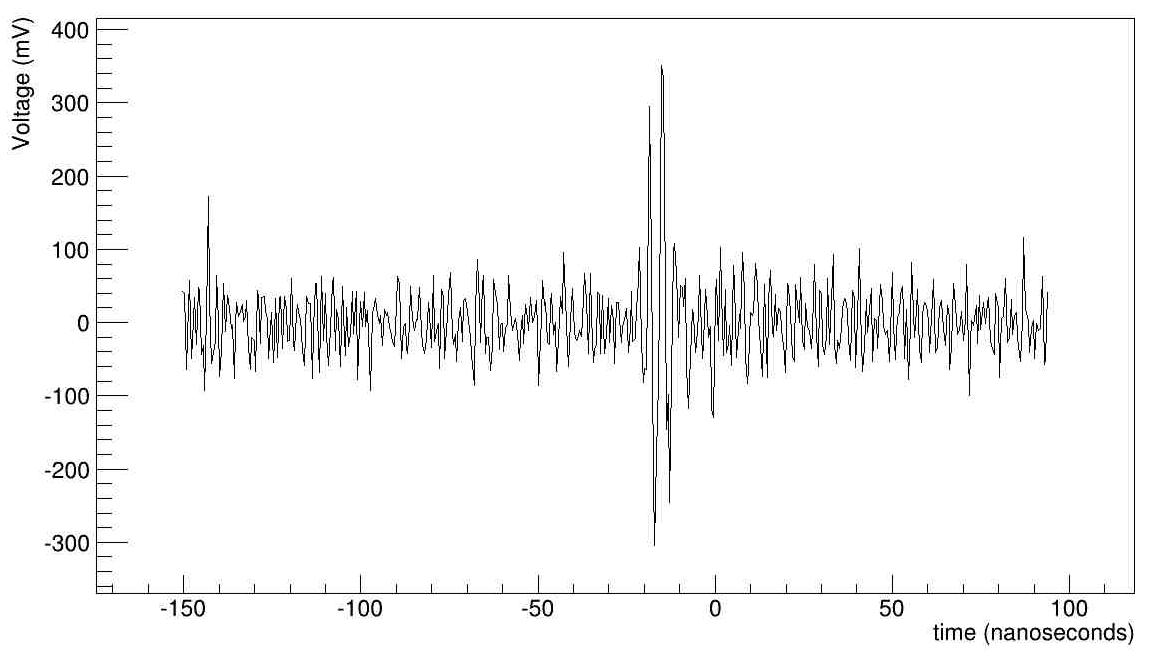
\includegraphics[width=4cm]{wave_box}};
  
  \node[] at (4,0) (box2) {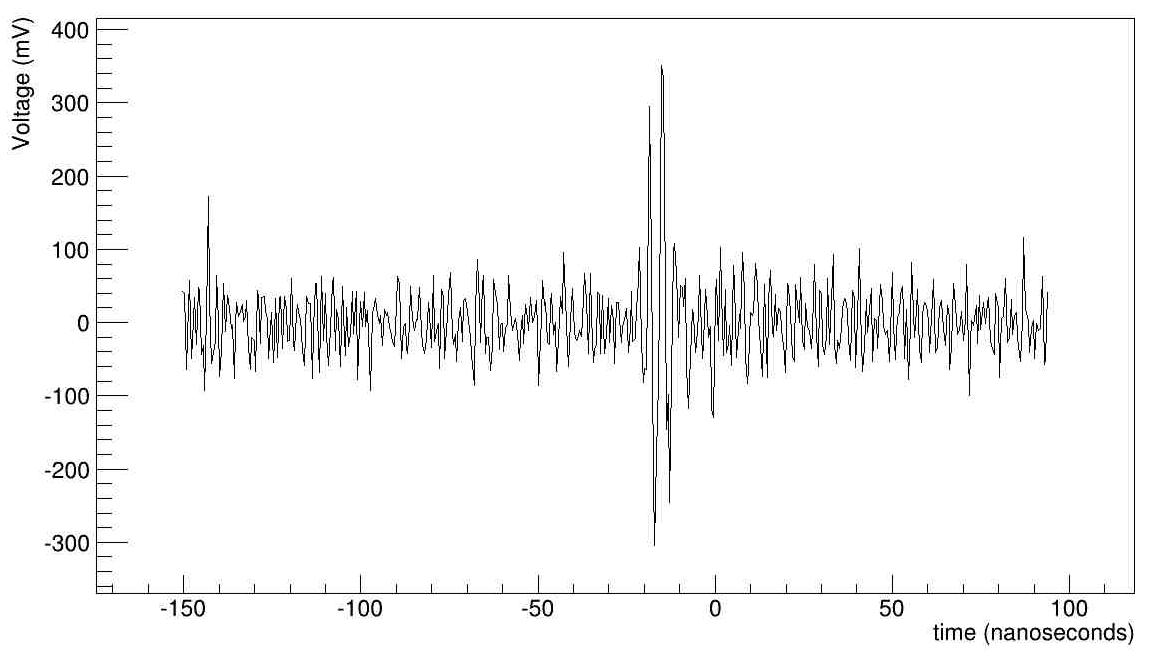
\includegraphics[width=4cm]{wave_box}};

  \node[] at (-4,0) (box2) {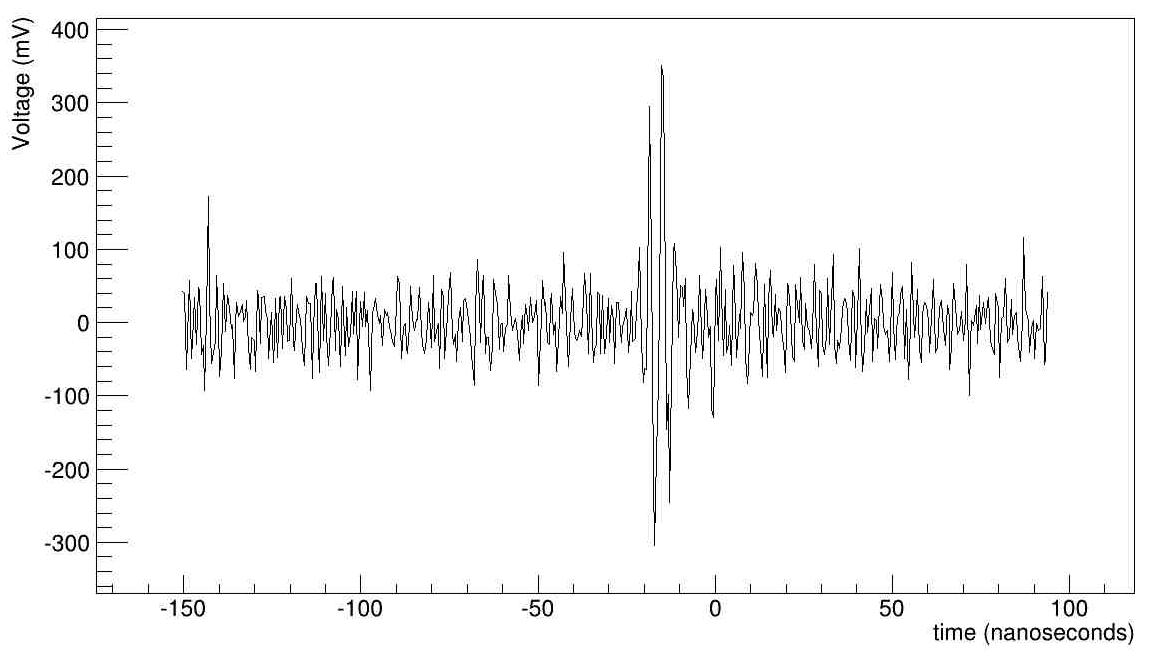
\includegraphics[width=4cm]{wave_box}};

  \draw[thick, red] (-5.3, -1.5) rectangle (-3.3, 1.5);

  \draw[thick, red] (5.3, -1.5) rectangle (3.3, 1.5);

  \draw[thick, red] (-1, -1.5) rectangle (1, 1.5);
  
  
  
 \end{tikzpicture}

 
 
 
 \caption{An example of different time windows for modes of \p{V MIMIC MODE} }
 
 \label{example v mimic mode}
 
 \end{centering}
 
 \room
 
 
\end{figure}


\newpage


\subsection{Other Parameters}\label{other parameters}

\pr{RANDOM MODE}=1. At mode 0 we get the same random seed every run. Useful for debugging. The default mode 1 generates a new random seed assuring randomly generated events. 

\pr{EVENT TYPE}=0 (default) for neutrinos. Future releases may include black holes or monopoles. 

\pr{LPM}=1. mode 0 no LPM effect. mode 1 (default) LPM effect is used. 

\room

These two functions decide the size and sample rate of the waveforms.

\pr{NFOUR}=1024. The number of bins in the fourier space waveform. This value must be some power of 2. The eventual waveform in time domain will have \p{NFOUR}/ 2 bins. 

\pr{TIMESTEP}=5E-10. The sampling rate for the channels. The defualt value is 5E-10, for 2 GHz sampling rate of actual digitizer. 

The time duration of the recorded waveforms we get is decided by:

\begin{equation*} T=N_\text{time domain} \times \Delta t \end{equation*}

\room 

where \p{NFOUR}= $2 N_\text{time domain}$ and \p{TIMESTEP}= $\Delta t$.

\room

\pr{WHICHPARAMETERIZATION}=0. Old definitions from icemc. Do not change this parameter. 

\pr{WAVE TYPE}=0 plane wave. used for ray tracing puproses. Do not change this parameter. 

\pr{PHASE}=90 in Degrees.  This is used to make the Fourier components imaginary. Do not change this parameter. 

\pr{TESTBED ON}=0 (default). mode 1 is the old implementation. Do not change this parameter.

\pr{CALPUL OFFCONE ANGLE}=35 degrees. Old definition for previous implementation of cal pulser. Do not change this parameter.

\pr{MAXT DIODE}=70E-9. Old parameter definition. Do not change this parameter.

\pr{IWINDOW DIODE}=4.E-9 / \p{TIMESTEP} default is 10. Do not change this parameter.

\pr{CONST MEANDIODE}=-6.5e-15 unused debugging parameter. Do not change this parameter.

\pr{CONST RMSDIODE}=1.346e-13 unused debugging parameter. Do not change this parameter.

\pr{IDELAYBEFOREPEAK DIODE}=13.E-9 / \p{TIMESTEP} defualt is 33. Do not change this parameter.

\newpage

\section{Incompatibilities and other pitfalls}\label{pitfalls}

Here is a short (and not comprehensive) list of problems that we may run into while using \arasim. Hopefully this will save some time debugging common errors in running and analysing simulations. 

\subsection{Incompatible settings}

One common problem is using one mode of \arasim that does not work with another setting. The most frequent example is using testbed parameters with non-testbed \p{DETECTOR} modes. Although \arasim makes a check to prevent such problems a diligent user may still find ways to crash the program or to get strange results. 

A good habit is to keep distinct setup files with settings for testbed (which are tweaked as necessary), a seperate file for ideal detector(s), and so on for each commonly used variety of simulation. 

\begin{itemize}

\item A common issue is with \tb{testbed only} parameters. A list of such parameters is given:

\begin{itemize}

 \item \p{NOISE TEMP MODE}= 1
 
 \item \p{TRIG ONLY BH ON}= 1
 
 \item \p{USE CH GAINOFFSET}= 1
 
 \item \p{USE TESTBED RFCM ON}= 1
 
 \item \p{RFCM GAINOFFSET} only checked if the above mode is used. 
 
 \item \p{READGEOM}= 1
 
 \item \p{CALPULSER ON} $>0$
 
 \item \p{CALPUL AMP} only checked if the above mode is used. 
  
 \item \p{V MIMIC MODE} $>0$
 
\end{itemize}


\item Some parameter changes that should be made when working with a detector array (when using \p{DETECTOR}= 1 with \p{number of stations} $>1$) or with \p{DETECTOR}= 2:

\begin{itemize}

 \item In `pick near' mode, make sure the radius given in \p{POSNU RADIUS} is large enough to contain the whole array. 
 
 \item In such cases the \p{RAYSOL RADIUS} may be smaller than \p{POSNU RADIUS}.
 
 
 
\end{itemize}

\item Although the `pick near' function (\p{INTERACTION MODE}= 1) is very useful for running shorter simulations, using `pick unbiased' (\p{INTERACTION MODE}= 0) may be more accurate when trying to simulate the real results of an experiment in Antarctica. Some issues may arise though:

\begin{itemize}

 \item Since many neutrinos will be generated outside the \p{RAYSOL RADIUS}, it may take a long while before any of them triggers the detector. Increasing this radius will not necessarily make things better, as it will only incur more calls to the ray solver, for events that are hopelessly far away. 
 
 \item Using low energy spectra or small detector arrays will also reduce the number of triggered events (remember that even ARA37 is estimated to detect a handful of events a year).
 
 \item In cases of low trigger rate we may get empty output trees (if working in \p{ONLY PASSED EVENTS}= 0) or an indefinitely long runtime (in \p{ONLY PASSED EVENTS}= 1).
 
\end{itemize}

\end{itemize}


\subsection{Problems running AraSim}

Here are some tips and known problems one may run into using \arasim. 

\begin{itemize}
 
 \item When simulation is finished we still need to do some analysis on the `outputs/AraOut.root' file. Some common issues are:
 
 \begin{itemize}
  
  \item Is the file very small? Are you sure there were any global triggers? 
 
  \item Are the simulation parameters reasonable? Running \p{NNU}= 100 in `pick unbiased' mode will likely cause no triggers.
  
  \item Did you choose the right data save modes (see section \ref{writing events})?
  
  \item Did you load the right libraries (to read classes like Detector, Event, etc..)?
  
  \item Are you looking in the right tree? Remember:
  
  \begin{itemize}
  
  \item eventTree contains the ``realistic'' data from the detector (only the final waveforms and measureable quantities; 
  
  \item AraTree2 conatins the ``behind the scenes'' data on each event (position and energy of neutrinos, etc); and 
  
  \item AraTree contains the global run parameters like detector and neutrino spectrum used. 
  
  \end{itemize}
  
 \end{itemize}

 \item Simulation running too long. This usually happens in \p{ONLY PASSED EVENTS} = 1 where \arasim continues to run until the number of global triggers reachs \p{NNU PASSED}. 
 
 \begin{itemize}
 
%  \item In \p{ONLY PASSED EVENTS} = 1 simulation will continue until a set number of neutrinos pass the global trigger.
 
  \item Did you choose reasonable parameters? Running \p{NNU PASSED} = 100 in `pick unbiased' might take a \emph{very} long time. 
  
  \item Are you using reasonable energies and detector layout to be able to see any neutrinos?
  
  \item Are the neutrinos being generated inside the range of \p{RAYSOL RADIUS}? If not, simulation may run indefinately. 
  
  \item In \p{TRIG ANALYSIS MODE} = 2 triggering only runs on noise, so trigger rate may be very low (unless we change the threshold). 
  
  \item If run time is $<\infty$ but still too long, consider splitting simulation into several runs (see section \ref{running arasim}).
  
 \end{itemize}

 
\end{itemize}



\section{Additional Issues}

Some more explanations on some of the results we can get from \arasim. 

\subsection{Working with Weights}\label{weights}

working progress



\newpage

\section{Reference to AraSim parameters}
\hyphenchar\font=-1
\label{references}

\openup -2pt

\#\# // Setup file with basic notation. Please report any issues or mistakes:\\ (\url{guy.nir@weizmann.ac.il})\\ Date: \today // \#

\rsection{neutrino energies}

\r[19]{EXPONENT}{the energy spectrum of the neutrinos.}

\rsection{number of neutrinos}

\r{ONLY PASSED EVENTS}{ 0: runs \p{NNU} neutrinos. 1: runs until \p{NNU PASSED} neutrinos globally trigger.}

\r[100]{NNU}{The total number of neutrinos thrown.}

\r[10]{NNU PASSED}{when using \p{ONLY PASSED EVENTS} this determines how many events will pass the trigger.}

\r{OUTPUT TDR GRAPH}{saves this number of tunnel diode response waeforms.}


\rsection{generating noise}

\r[16]{NOISE EVENTS}{the number of noise wf generated.}

\r{NOISE WAVEFORM GENERATE MODE}{new noise wf are generated for each event. 1: old mode all noise wf are made beforehand.}

\r{NOISE}{0: flat thermal distribution. 1: calibrated Rayleigh noise }

\r{NOISE TEMP MODE}{0: same noise wf for all channels. 1: different temperatures for each channel. 2: diff temps for first 8 channels.}

\r[325]{NOISE TEMP}{if using thermal distribution, use this temperature (in Kelvins).}

\r[16384]{DATA BIN SIZE}{size of noise wf used to get noise floor (or to make all noise wf's before simulation when \p{NOISE WAVEFORM GENERATE MODE}=1. must be power of 2.}



\rsection{neutrino position}

\r[1]{INTERACTION MODE}{0: make nu's all over antarctica. 1: pick near (a cylinder around detector). 2: exact location at (353.55, 612.37, 707.1). 3: pick near-unbiased (a sphere around detector)}

\r[3000]{POSNU RADIUS}{radius around detector in pick near mode.}

\r[5000]{PICKNEARUNBIASED R}{spherical radius around detector in pick near-unbiased mode.}

\r{PICK POSNU DEPTH}{0: use all ice down to bedrock. 1: choose maximum depth yourself.}

\r{MAX POSNU DEPTH}{the maximum depth when \p{PICK POSNU DEPTH}=1.}

\r{NNU THIS THETA}{0: choose nutrino incident angle at random. 1: choose specfic angle range.}

\r{NNU THETA}{the angle chosen when \p{NNU THIS THETA}=1 is chosen. Use radians! }

\r{NNU D THETA}{the range around \p{NNU THETA} (up and down).}

\r[1]{SECONDARIES}{0: no secondary interactions. 1: allow secondary interactions.}

\r[1]{TAUDECAY}{0: do not allow secondary tau decay. 1: allow secondary decay of tau's, only works when \p{SECONDARIES}=1.}



\rsection{ray solving}

\r[5000]{RAYSOL RANGE}{distance from detector above which we do not attempt a ray solution (there is no trigger check beyond this).}



\rsection{triggering}

\r{USE INSTALLED TRIGGER SETTINGS}{0: ideal detector trigger settings. 1: use triggering as implemented in real stations (\tb{testbed only!}).}

\r{TRIG ANALYSIS MODE}{0: signal+noise. 1: signal only. 2: noise only}

\r[-6.15]{POWERTHRESHOLD}{the trigger threshold (the closer to zero the weaker the threshold. measured in sigmas above the noise floor.}

\r[1.1E-7]{TRIG WINDOW}{time window in which several channels must trigger to pass global trigger test.}

\r[1E-6]{TRIG TIMEOUT}{dead time for detector.} 

\r[1]{TRIG MODE}{0: trigger for N antennas of any kind. 1: trigger on either Nh Hpol or Nv Vpol antennas.}

\r[3]{N TRIG}{number of total antennas required for a global trigger (if \p{TRIG MODE}=0).}

\r[3]{N TRIG V}{number of Vpol required for a global trigger (if \p{TRIG MODE}=1).}

\r[3]{N TRIG H}{number of Hpol required for a global trigger (if \p{TRIG MODE}=1).}

\r[0]{TRIG SCAN MODE}{triggering algorithm. 0: old code. 1: new, faster code. 2: scan all powerthreshold values. 3: save single channel trigger powerthreshold values, too. }


\r{TRIG ONLY BH ON}{0: check trigger on all channels. 1: check only borehole antennas.}

\r{TRIG THRES MODE}{0: use same threshold for all channels. 1: use seperate thershold for each channel using 'data/thresholdoffset.csv'.}

\r{USE MANUAL GAINOFFSET}{0: pass control to \p{USE CH GAINOFFSET} below. 1: add a single value to the offset of all channels.}

\r{MANUAL GAINOFFSET VALUE}{is the offset to the threshold when using \p{USE MANUAL GAINOFFSET}=1}

\r{USE CH GAINOFFSET}{0: use no gain offsets. 1: use specfic gain offsets for each channel using 'data/preampgainoffsets.csv' (\tb{testbed only!})}

\r{USE TESTBED RFCM ON}{0: don't apply specific amplification offsets. 1: use measured TB data to cancel amplification gain.}

\r[80]{RFCM OFFSET}{when \p{USE TESTBED RFCM ON}=0 use this value to cancel the amplification gain of electronic components.}



\rsection{ice and earth}

\r{CONSTANTCRUST}{This is a left over parameter, do not change these settings.}

\r{CONSTANTICETHICKNESS}{This is a left over parameter, do not change these settings.}

\r{FIXEDELEVATION}{Elevation fixed to the thickness of the ice. Don't change this setting.}

\r{MOOREBAY}{which attenuation length measurements to use. 0: south pole data. 1: Moore's Bay measurements.}

\r[1]{ATMOSPHERE}{0: no atmosphere (not recommended). 1: use atmosphere (default).}

\r{ICE MODEL}{0: Crust 2.0 or 1: bedmap (old ice model).}

\r[1]{NOFZ}{0: constant index of refraction (not recommended). 1: n changes with depth (default).}

\r{GETCHORD MODE}{which code to use for weights of nu's passing the earth / atmosphere. 0: old code.  1: new untested code.}

\r{taumodes}{0: no tau modes. 1: allow tau nu's interaction in bedrock to create tau's. works only when \p{GETCHORD MODE}=1.}



\rsection{detector layout}

\r[1]{DETECTOR}{0: unused. 1: ideal ARA station. can choose 1 to 7 stations. 2: large array in hexagonal design. 3: testbed.}

\r[1]{number of stations}{number of stations used in \p{DETECTOR}=1 mode. }

\r[2000]{station spacing}{separation between stations in modes 1 and 2. in meters.}

\r[4]{stations per side}{number of stations on a side of the hexagon in \p{DETECTOR}=2 mode. for N on a side get 3N(N-1)+1 stations.} 

\r[10000]{core x}{location of array in global coordinates, used to avoid the bin crossing of 2degree bins.}

\r[10000]{core y}{same as above.}

\r[4]{number of strings per station}{number of strings on an ideal station.}

\r[10]{R string}{distance of string poisitions from center of station. in meters.}

\r{BORE HOLE ANTENNA LAYOUT}{order of antennas on the string. 0: HVHV. 1: VHV. 2: VVHV. 3: HHHV. 4: HHV.}

\r[200]{z max}{lowest antenna position on the string. in meters depth}

\r[1]{BH ANT SEP DIST ON}{0: all distances are the same (choose \p{z btw}). 1: choose each distance youself (use \p{z btwAB}).}

\r[10]{z btw}{single distance for all BH antennas, used when \p{BH ANT SEP DIST ON}= 0}

\r[2]{z btw01}{distance between lowest antenna and next one. in meters}

\r[15]{z btw12}{distance between second and third antenna.}

\r[2]{z btw23}{distance between third and last (uppermost) antenna.}

% \r{TRIGGER ONLY BH ON}{0: use all antennas to trigger. 1: use only borehole antennas (first 8).}

\r{READGEOM}{0: use idealized detector layout. 1: read from sqlite file. TB ONLY!}

\r{CALPULSER ON}{0: no calpulser. 1: use 2012 pulser. 2: use 2011 Vpol. 3: use 2011 Hpol. 4: use both V and H pol, average location of pulser. TB ONLY!}

\r[0.15]{CALPUL AMP}{amplitude modifier for the calpulser, to match the power of real pulser}. 



\rsection{writing events}

\r{DATA SAVE MODE}{0: save waveforms and primitive spectra to AraTree2 (include spectra at different stages of simulation). 1: save only waveforms after trigger. 2: save just physics data per event.}

\r{WRITE ALL EVENTS}{0: save only triggered events to eventTree (realistic case). 1: fill eventTree with all events (untriggered give zero wf graphs) 2: write nothing (leave eventTree empty)}

\r{FILL TREE MODE}{0: save all events to AraTree2 (triggered or not) 1: don't save events outside of ice (in pick unbiased mode) 2: save just triggered events.}

\r{V MIMIC MODE}{0: save wavforms using standard time window. 1: use offsets from data to get real time windows (TB ONLY!). 2: add manual offsets to thos in 1 (TB ONLY!).}
\rsection{other parameters}

\r[1]{RANDOM MODE}{0: same random seed (debugging). 1: new random seed for simulations}

\r{SIMULATION MODE}{0: frequency domain. 1: time domain simulation}

\r{EVENT TYPE}{0: neutrinos. other modes in future release.}

\nopagebreak
\r[1]{LPM}{0: don't use LPM effect. 1: use LPM (default)}

\nopagebreak
\r[1024]{NFOUR}{Fourier space sample size. Twice the number of bins in time domain wf. must be power of 2.}

\nopagebreak
\r[5E-10]{TIMESTEP}{sample rate for digitizer. decides the time difference between data points in wf.}



\rs{WHICHPARAMETERIZATION}{}

\rs{WAVE TYPE}{}

\rs{PHASE}{}

\rs{TESTBED ON}{}

\rs{CALPUL OFFCONE ANGLE}{}

\rs{MAXT DIODE}{}

\rs{IWINDOW DIODE}{}

\rs{CONST MEANDIODE}{}

\rs{CONST RMSDIODE}{}

\rs{IDELAYBEFOREPEAK}{}






\end{document}
